\documentclass[10pt,a4paper]{article}
\usepackage[margin=18mm,top=22mm,bottom=18mm,headsep=7mm,footskip=9mm]{geometry}
\usepackage{fontspec,amsmath,amssymb,array,tabularx,xcolor,tikz,fancyhdr,hyperref}
\usetikzlibrary{arrows.meta}
\setmainfont{NotoSansKR-Regular.ttf}[Path=../../assets/fonts/,BoldFont=NotoSansKR-Semibold.ttf]
\newfontfamily\brandfont{NotoSansKR-Regular.ttf}[Path=../../assets/fonts/,BoldFont=NotoSansKR-Semibold.ttf]
\definecolor{ink}{HTML}{25343D}
\definecolor{accent}{HTML}{216B7A}
\definecolor{muted}{HTML}{637078}
\definecolor{grid}{HTML}{D9E0E3}
\definecolor{soft}{HTML}{F2F6F6}
\definecolor{vectorblue}{HTML}{266CA8}
\definecolor{vectorteal}{HTML}{278276}
\definecolor{answerred}{HTML}{C42030}
\newif\ifanswers
\answerstrue
\hypersetup{colorlinks=true,urlcolor=accent,pdftitle={OZ Lab AI Study: Linear Algebra Visual Quiz Answer Key},pdfauthor={OZ Lab}}
\setlength{\parindent}{0pt}
\setlength{\parskip}{2pt}
\setlength{\headheight}{21pt}
\setlength{\tabcolsep}{3pt}
\renewcommand{\arraystretch}{1.25}
\pagestyle{fancy}\fancyhf{}
\fancyhead[L]{\brandfont\fontsize{8}{10}\selectfont\bfseries\color{ink}OZ Lab\quad AI Study}
\fancyhead[R]{\brandfont\fontsize{7.5}{10}\selectfont\color{muted}Linear Algebra\quad /\quad Visual Check}
\fancyfoot[L]{\brandfont\fontsize{7}{9}\selectfont\color{muted}3BLUE1BROWN\quad /\quad ESSENCE OF LINEAR ALGEBRA}
\fancyfoot[R]{\brandfont\fontsize{8}{10}\selectfont\color{ink}0\thepage\quad{\color{muted}/\ 03}}
\renewcommand{\headrulewidth}{.3pt}
\renewcommand{\headrule}{\hbox to\headwidth{\color{grid}\leaders\hrule height\headrulewidth\hfill}}
\newcommand{\vc}[2]{\begingroup\renewcommand{\arraystretch}{1}\begin{bmatrix}#1\\#2\end{bmatrix}\endgroup}
\newcommand{\mat}[4]{\begingroup\renewcommand{\arraystretch}{1}\begin{bmatrix}#1&#2\\#3&#4\end{bmatrix}\endgroup}
\newcommand{\sect}[2]{\par\vspace{3mm}{\brandfont\fontsize{10}{15}\selectfont\bfseries\color{accent}#1}\quad{\fontsize{14}{18}\selectfont\bfseries\color{ink}#2}\par\vspace{3mm}}
\newcommand{\q}[2]{\par\noindent\makebox[7mm][l]{\brandfont\fontsize{10}{14}\selectfont\bfseries\color{accent}#1}\begin{minipage}[t]{\dimexpr\linewidth-7mm}\fontsize{9.5}{14}\selectfont #2\end{minipage}\par\vspace{1mm}}
\newcommand{\given}[1]{\par\hspace*{7mm}{\fontsize{10}{15}\selectfont$\displaystyle #1$}\par\vspace{1mm}}
\newcommand{\opt}[3]{{\leavevmode\ifanswers\ifnum#1=#2\color{answerred}\fi\fi(#1)\enspace #3}}
\newcommand{\choices}[5]{\par\hspace*{7mm}\begin{minipage}{\dimexpr\linewidth-7mm}\fontsize{9}{13}\selectfont\begin{tabularx}{\linewidth}{@{}X X@{}}\opt{1}{#1}{#2}&\opt{2}{#1}{#3}\\[4mm]\opt{3}{#1}{#4}&\opt{4}{#1}{#5}\end{tabularx}\end{minipage}\par}
\newcommand{\stackchoices}[5]{\par\hspace*{7mm}\begin{minipage}{\dimexpr\linewidth-7mm}\fontsize{9}{13.5}\selectfont{\opt{1}{#1}{#2}}\par{\opt{2}{#1}{#3}}\par{\opt{3}{#1}{#4}}\par{\opt{4}{#1}{#5}}\end{minipage}\par}
\newcommand{\solution}[2]{\par\vspace{1mm}\hspace*{7mm}\begin{minipage}[t][#1][t]{\dimexpr\linewidth-7mm}\vspace{0pt}\fontsize{8.3}{12}\selectfont\ifanswers\leavevmode\color{answerred}#2\else{\color{grid}\hrule height .3pt}\fi\end{minipage}\par}
\newcommand{\sep}{\vspace{3mm}{\color{grid}\hrule height .25pt}\vspace{3mm}}
\newcommand{\smallaxes}{
  \draw[grid,line width=.2pt,step=1] (-2,-2) grid (2,2);
  \draw[-{Stealth[length=1.4mm]},ink,line width=.4pt] (-2.25,0)--(2.25,0);
  \draw[-{Stealth[length=1.4mm]},ink,line width=.4pt] (0,-2.25)--(0,2.25);
}
\newcommand{\spanplot}[1]{\begin{tikzpicture}[x=.62cm,y=.62cm,baseline=(current bounding box.center)]
  \path[use as bounding box] (-2.45,-2.45) rectangle (2.45,2.45);
  \ifnum#1=1\fill[accent!12] (-2,-2) rectangle (2,2);\fi
  \smallaxes
  \ifnum#1=2\draw[-{Stealth[length=2mm]},accent,line width=1pt] (0,0)--(2.15,2.15);\fill[accent] (0,0) circle(1.4pt);\fi
  \ifnum#1=3\draw[accent,line width=1pt] (0,0)--(1.6,1.6);\fill[accent] (0,0) circle(1.4pt);\fill[accent] (1.6,1.6) circle(1.4pt);\fi
  \ifnum#1=4\draw[{Stealth[length=2mm]}-{Stealth[length=2mm]},accent,line width=1pt] (-2.15,-2.15)--(2.15,2.15);\fi
  \ifanswers\ifnum#1=4\draw[answerred,line width=.8pt] (-2.4,-2.4) rectangle (2.4,2.4);\fi\fi
\end{tikzpicture}}
\AtBeginDocument{\fontsize{9.5}{14}\selectfont\color{ink}}
\begin{document}

{\brandfont\fontsize{19}{24}\selectfont\bfseries Linear Algebra\par}
\vspace{1mm}
{\fontsize{11}{16}\selectfont Vectors, matrices, and dot products}\hfill{\ifanswers\color{answerred}\bfseries Worked answers\else\color{muted}Concept check\fi}\par
\vspace{3mm}
{\fontsize{8}{12}\selectfont\color{muted}Name\quad\rule{34mm}{.3pt}\hfill Date\quad\rule{28mm}{.3pt}}\par
\vspace{2mm}
{\fontsize{8}{12}\selectfont\color{muted}Choose one answer per question\quad ·\quad Use the margins for calculations and sketches\quad ·\quad 25 minutes}
\sect{01}{Vectors and Span}

\q{1}{Why should we understand \textbf{how space changes}, as well as calculate with matrices?}
\stackchoices{2}
{A diagram always lets us skip exact numerical calculations}
{It helps us interpret a calculation and decide which operation to use}
{It shows that every matrix performs the same rotation}
{Geometry is unrelated to calculation and can be memorized separately}
\solution{10mm}{Answer (2)\quad Calculations give a result; geometry helps explain what the operation means and when to use it}
\sep

\q{2}{\textbf{Calculate and draw} $\mathbf r=2\mathbf u-\mathbf v$ on the grid\quad Choose its coordinates}
\begin{minipage}[t]{.59\linewidth}
\given{\mathbf u=\vc{1}{2},\qquad \mathbf v=\vc{-1}{1}}
\vspace{2mm}
\choices{3}{$\vc{1}{3}$}{$\vc{3}{5}$}{$\vc{3}{3}$}{$\vc{1}{5}$}
\vspace{2mm}
\solution{19mm}{Answer (3)\quad $2\mathbf u-\mathbf v=(2,4)-(-1,1)=(3,3)$\\Subtracting a negative is the same as adding a positive}
\end{minipage}\hfill
\begin{minipage}[t]{.37\linewidth}\vspace{0pt}\centering
\begin{tikzpicture}[x=.62cm,y=.62cm]
\path[use as bounding box] (-2.7,-1.5) rectangle (4.7,5.4);
\draw[grid,line width=.25pt,step=1] (-2,-1) grid (4,5);
\draw[-{Stealth[length=1.7mm]},line width=.5pt] (-2.3,0)--(4.35,0) node[right]{\scriptsize$x$};
\draw[-{Stealth[length=1.7mm]},line width=.5pt] (0,-1.2)--(0,5.2) node[above]{\scriptsize$y$};
\foreach \x in {-2,1,2,3,4}{\node[below,fill=white,inner sep=.7pt] at (\x,0){\tiny$\x$};}
\foreach \y in {1,2,3,4,5}{\node[left,fill=white,inner sep=.7pt] at (0,\y){\tiny$\y$};}
\node[below left] at (0,0){\tiny$0$};
\draw[-{Stealth[length=2mm]},vectorblue,line width=1pt] (0,0)--(1,2) node[above right]{\small$\mathbf u$};
\draw[-{Stealth[length=2mm]},vectorteal,line width=1pt] (0,0)--(-1,1) node[above left]{\small$\mathbf v$};
\ifanswers
\draw[dashed,answerred!65,line width=.65pt] (1,2)--(2,4)--(3,3);
\draw[-{Stealth[length=2mm]},answerred,line width=1pt] (0,0)--(3,3);
\fill[answerred] (3,3) circle(1.6pt);
\node[answerred,above right,fill=white,inner sep=1pt] at (3,3){\scriptsize$\mathbf r$};
\fi
\end{tikzpicture}
\end{minipage}
\sep

\q{3}{As $a,b$ range over \textbf{all real numbers}, which set contains every possible vector endpoint?}
\given{\mathbf u=\vc{1}{1},\quad\mathbf v=\vc{2}{2},\qquad \operatorname{Span}(\mathbf u,\mathbf v)=\{a\mathbf u+b\mathbf v\mid a,b\in\mathbb R\}}
\vspace{2mm}
\begin{tabularx}{\linewidth}{@{}*{4}{>{\centering\arraybackslash}X}@{}}
\spanplot{1}&\spanplot{2}&\spanplot{3}&\spanplot{4}\\
{\fontsize{8.5}{12}\selectfont\opt{1}{4}{The entire plane}}&{\fontsize{8.5}{12}\selectfont\opt{2}{4}{A positive ray}}&{\fontsize{8.5}{12}\selectfont\opt{3}{4}{A line segment}}&{\fontsize{8.5}{12}\selectfont\opt{4}{4}{An infinite line}}
\end{tabularx}
\solution{14mm}{Answer (4)\quad $\mathbf v=2\mathbf u$, so $a\mathbf u+b\mathbf v=(a+2b)\mathbf u$\\Negative multiples are allowed, giving the whole line $y=x$ through the origin in both directions}

\newpage
\sect{02}{Basis and Linear Transformations}

\q{4}{Which set of vectors can be a \textbf{basis for the entire plane}?}
\choices{1}
{$\vc{1}{0},\ \vc{1}{1}$}
{$\vc{1}{2},\ \vc{2}{4}$}
{$\vc{1}{0},\ \vc{0}{0}$}
{$\vc{1}{0},\ \vc{0}{1},\ \vc{1}{1}$}
\solution{14mm}{Answer (1)\quad The two nonparallel vectors span the plane without redundancy\\In (4), the third vector is the sum of the first two: the set spans the plane but is not a basis}
\sep

\q{5}{Which is a \textbf{linear transformation}?}
\given{T(a\mathbf u+b\mathbf v)=aT(\mathbf u)+bT(\mathbf v)}
\choices{3}
{$T(x,y)=(x+1,\ y)$}
{$T(x,y)=(x^2,\ y)$}
{$T(x,y)=(2x,\ x+y)$}
{$T(x,y)=(x,\ |y|)$}
\solution{17mm}{Answer (3)\quad It preserves addition and multiplication by a real number\\(1) moves the origin; in (2), doubling $x$ quadruples $x^2$\\(4) has $T(0,-1)\ne -T(0,1)$, so it does not preserve negative multiples}
\sep

\q{6}{A linear transformation $T$ moves the two basis vectors as shown\quad Choose \textbf{its matrix $A$}}
\begin{minipage}[t]{.63\linewidth}
\given{T\!\left(\vc{1}{0}\right)=\vc{1}{1},\qquad T\!\left(\vc{0}{1}\right)=\vc{-1}{2}}
\vspace{2mm}
\choices{2}{$\mat{1}{1}{-1}{2}$}{$\mat{1}{-1}{1}{2}$}{$\mat{-1}{1}{2}{1}$}{$\mat{1}{0}{0}{1}$}
\end{minipage}\hfill
\begin{minipage}[t]{.34\linewidth}\vspace{0pt}\centering
\begin{tikzpicture}[x=.65cm,y=.65cm]
\path[use as bounding box] (-2.5,-1.6) rectangle (4,3.4);
\draw[grid,line width=.25pt,step=1] (-2,-1) grid (3,3);
\draw[-{Stealth[length=1.7mm]},line width=.5pt] (-2.3,0)--(3.5,0) node[right]{\scriptsize$x$};
\draw[-{Stealth[length=1.7mm]},line width=.5pt] (0,-1.3)--(0,3.2) node[above]{\scriptsize$y$};
\foreach \x in {-2,-1,1,2,3}{\node[below,fill=white,inner sep=.7pt] at (\x,0){\tiny$\x$};}
\foreach \y in {1,2,3}{\node[left,fill=white,inner sep=.7pt] at (0,\y){\tiny$\y$};}
\node[below left] at (0,0){\tiny$0$};
\draw[-{Stealth[length=2mm]},vectorblue,line width=1pt] (0,0)--(1,1) node[above right]{\scriptsize$T(\mathbf e_1)$};
\draw[-{Stealth[length=2mm]},vectorteal,line width=1pt] (0,0)--(-1,2) node[above left]{\scriptsize$T(\mathbf e_2)$};
\ifanswers
\draw[-{Stealth[length=2mm]},answerred,line width=1pt] (0,0)--(3,0);
\fill[answerred] (3,0) circle(1.6pt);
\node[answerred,above,fill=white,inner sep=1pt] at (2.5,.12){\scriptsize$T(\mathbf v)$};
\fi
\end{tikzpicture}
\end{minipage}
\solution{10mm}{Answer (2)\quad The first column is $T(\mathbf e_1)$; the second is $T(\mathbf e_2)$\quad $\mathbf e_1=(1,0),\ \mathbf e_2=(0,1)$}
\sep

\q{7}{Apply $T$ from Question 6 to $\mathbf v$\quad \textbf{Plot $T(\mathbf v)$ on the grid above} and choose its coordinates}
\given{\mathbf v=\vc{2}{-1},\qquad T(\mathbf v)=2T(\mathbf e_1)-T(\mathbf e_2)}
\choices{4}{$\vc{1}{-4}$}{$\vc{1}{0}$}{$\vc{3}{4}$}{$\vc{3}{0}$}
\solution{16mm}{Answer (4)\quad $T(\mathbf v)=2(1,1)-(-1,2)=(3,0)$\\Use the same original coefficients $2,-1$ with the transformed basis vectors}

\newpage
\sect{03}{Composition and Dot Products}

\q{8}{Apply \textbf{$A$ first, then $B$} to $\mathbf x$\quad Choose the correct combined matrix and result}
\given{A=\mat{1}{1}{0}{1},\qquad B=\mat{0}{-1}{1}{0},\qquad \mathbf x=\vc{1}{1}}
\choices{1}
{$BA$,\quad result $\vc{-1}{2}$}
{$AB$,\quad result $\vc{-1}{2}$}
{$BA$,\quad result $\vc{0}{1}$}
{$AB$,\quad result $\vc{0}{1}$}
\vspace{2mm}
\given{\mathbf x\ \xrightarrow{\ A\ }\ \underbrace{\hspace{22mm}}_{\text{intermediate}}\ \xrightarrow{\ B\ }\ \underbrace{\hspace{22mm}}_{\text{final result}}}
\solution{14mm}{Answer (1)\quad $A\mathbf x=(2,1)$,\quad $B(A\mathbf x)=(-1,2)$\quad The combined matrix is $BA$\\Reversing the order gives $A(B\mathbf x)=(0,1)$, a different result}
\sep

\q{9}{\textbf{Draw a perpendicular} from the tip of $\mathbf w$ to the line through $\mathbf v$\quad Choose the projection length and dot product}
\begin{minipage}[t]{.59\linewidth}
\given{\mathbf v=\vc{2}{0},\qquad\mathbf w=\vc{3}{2}}
\given{\mathbf v\cdot\mathbf w=v_1w_1+v_2w_2}
\vspace{2mm}
\choices{3}
{Projection length $3$,\quad dot product $3$}
{Projection length $2$,\quad dot product $4$}
{Projection length $3$,\quad dot product $6$}
{Projection length $2$,\quad dot product $6$}
\end{minipage}\hfill
\begin{minipage}[t]{.37\linewidth}\vspace{0pt}\centering
\begin{tikzpicture}[x=.93cm,y=.93cm]
\path[use as bounding box] (-.6,-.8) rectangle (4.2,3.0);
\draw[grid,line width=.25pt,step=1] (0,0) grid (4,2.5);
\draw[-{Stealth[length=1.7mm]},line width=.5pt] (-.25,0)--(4,0) node[right]{\scriptsize$x$};
\draw[-{Stealth[length=1.7mm]},line width=.5pt] (0,-.3)--(0,2.65) node[above]{\scriptsize$y$};
\foreach \x in {1,2,3}{\node[below] at (\x,0){\tiny$\x$};}
\foreach \y in {1,2}{\node[left] at (0,\y){\tiny$\y$};}
\node[below left] at (0,0){\tiny$0$};
\draw[-{Stealth[length=2mm]},vectorblue,line width=1.2pt] (0,0)--(2,0) node[above]{\small$\mathbf v$};
\draw[-{Stealth[length=2mm]},vectorteal,line width=1pt] (0,0)--(3,2) node[above right]{\small$\mathbf w$};
\ifanswers
\draw[dashed,answerred,line width=.8pt] (3,2)--(3,0);
\draw[answerred,line width=.6pt] (2.8,0)--(2.8,.2)--(3,.2);
\fill[answerred] (3,0) circle(1.7pt);
\draw[answerred,{Stealth[length=1.5mm]}-{Stealth[length=1.5mm]}] (0,-.45)--(3,-.45) node[midway,below]{\scriptsize$3$};
\fi
\end{tikzpicture}
\end{minipage}
\solution{13mm}{Answer (3)\quad Projection length $3$;\quad $\mathbf v\cdot\mathbf w=2\times3+0\times2=6$\\Here the dot product is the projection length times $\lVert\mathbf v\rVert=2$, not the projection length alone}
\sep

\q{10}{A linear map $L$ sends \textbf{a vector to one number}\quad For $L(\mathbf x)=\mathbf w\cdot\mathbf x$, choose the correct $\mathbf w$ and result}
\given{\mathbf x=\vc{3}{1},\qquad L\!\left(\vc{1}{0}\right)=2,\qquad L\!\left(\vc{0}{1}\right)=-1}
\choices{2}
{$\mathbf w=\vc{-1}{2}$,\quad result $-1$}
{$\mathbf w=\vc{2}{-1}$,\quad result $5$}
{$\mathbf w=\vc{2}{-1}$,\quad result $\vc{6}{-1}$}
{$\mathbf w=\vc{2}{1}$,\quad result $7$}
\solution{17mm}{Answer (2)\quad $\mathbf w=(2,-1)$ and $L(\mathbf x)=2x_1-x_2$, so $L(3,1)=6-1=5$\\Duality here means that one vector $\mathbf w$ represents a linear map to a number\\In ML, $f_{\mathbf w}(\mathbf x)=\mathbf w\cdot\mathbf x$ with $b=0$ has the same form}
\vfill
{\fontsize{6.7}{9.5}\selectfont\color{muted}
Scope\quad Six 3Blue1Brown videos · Questions and diagrams created separately\\
\href{https://www.youtube.com/watch?v=ic_hG2M2nG0}{Visual intuition}\quad
\href{https://www.youtube.com/watch?v=ArgTeYVuJUo}{Vectors}\quad
\href{https://www.youtube.com/watch?v=2CcCOgDilO8}{Linear combinations, span, basis}\quad
\href{https://www.youtube.com/watch?v=35ESC-g49fY}{Transformations and matrices}\quad
\href{https://www.youtube.com/watch?v=gXjCxYuEybQ}{Composition}\quad
\href{https://www.youtube.com/watch?v=zSd7jd2HGhM}{Dot products and duality}\\
Content reference\quad
\href{https://github.com/3b1b/captions/blob/main/2016/eola-preview/english/transcript.txt}{Official introduction transcript}\quad
\href{https://www.3blue1brown.com/lessons/vectors/}{Vectors}\quad
\href{https://www.3blue1brown.com/lessons/span/}{Span}\quad
\href{https://www.3blue1brown.com/lessons/linear-transformations/}{Transformations}\quad
\href{https://www.3blue1brown.com/lessons/matrix-multiplication/}{Composition}\quad
\href{https://www.3blue1brown.com/lessons/dot-products/}{Dot Products}}
\end{document}
